\pagenumbering{arabic}
\setcounter{page}{37}
\chapter{Expected Outcome}
The main aim of this proposed system is to streamline the process of manga colourization making it fully automatic, overcoming the shortcomings of previous colorization models and architectures such as conditional GANs\cite{10.1007/978-3-030-72610-2_17}, pix2pix\cite{isola2018imagetoimage} and style2paints\cite{ACPR2017ZLM} by reducing monotonicity and eradicating the need to provide manual color hints.\\

Ideally, our model should produce colored outputs that closely resemble those hand-painted by a human artist. However, acknowledging the complexities involved, we anticipate our model achieving results that are visually comparable to, or surpass the quality of existing semi-automatic and automatic models. It is  important to note that the subjective nature of art allows for a spectrum of color interpretations; thus, while unconventional color choices may seem unrealistic, they are not inherently incorrect. For instance, a tree painted red can still evoke artistic merit within a specific style or context. \\

Given this consideration, it's crucial to recognize that the absence of contextual understanding within the text could lead to unintended outcomes. For instance, in a scenario where a manga text describes a "bright green bird," the model might erroneously color the bird white if it lacks contextual awareness and hasn't been exposed to a diverse range of bird illustrations in its training dataset.

\begin{figure}[htbp]
    \centering
    \begin{subfigure}[b]{0.48\textwidth}
        \includegraphics[width=\textwidth]{img/expected_bw.png}
        \caption{Black and white manga cover}
      
    \end{subfigure}
    \hfill
    \begin{subfigure}[b]{0.48\textwidth}
        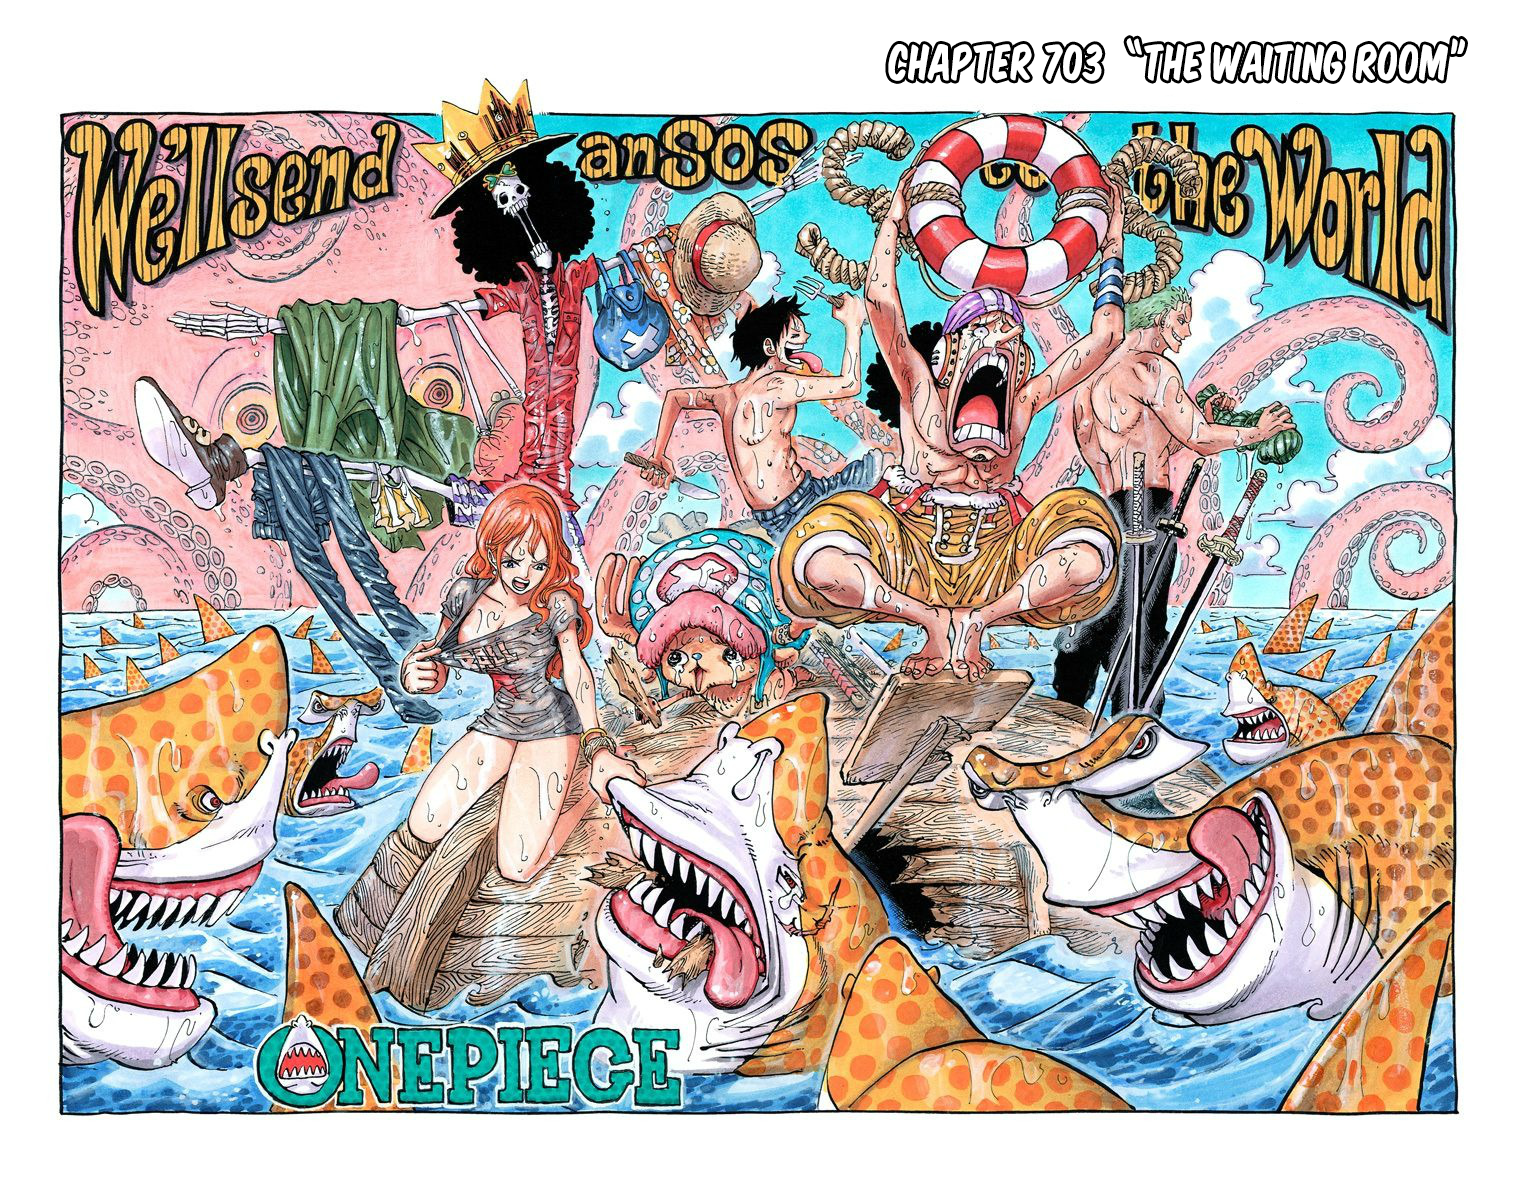
\includegraphics[width=\textwidth]{img/expected_human-drawn_ideal.png}
        \caption{human-colored manga cover}

    \end{subfigure}
    
\caption{Expected outcome for ideal automatic colorizer}
\label{fig:bad_images}
    
\end{figure}
\pagebreak